\chapter{Basics of Motor control} \label{Basics_motor_control}

\section{PWM speed control}
\begin{itemize}
    \item A pulse width modulation speed control system works by sending a series of "ON-OFF" pulses to the motor. The frequency of square wave is kept constant while varying the duty cycle (the fraction of time that the output voltage is “ON” compared to when it is "OFF").
    \item By changing the width of the ON duration, one can control the average DC voltage applied to the motor. 
    \item In other words, the wider the pulse width, the more average voltage applied to the motor terminals, the stronger the magnetic flux inside the armature windings and the faster the motor will rotate.
    \item Larger the duty-cycle, the faster the motor will rotate. Similarly, shorter the duty-cycle, the slower the motor will rotate.
\end{itemize}

\begin{figure}[h!]
\centering
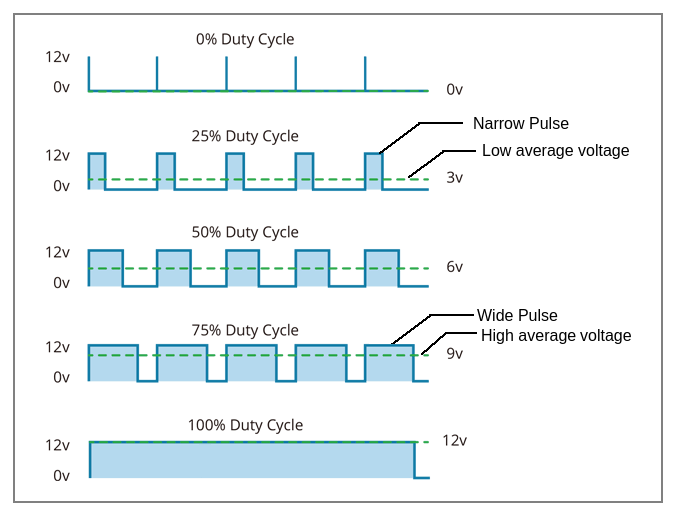
\includegraphics[width=9cm]{./Figures/PWM_speed_control.png}
\caption{PWM speed control}
\label{BLDC_runner}
\end{figure}

\section{Brushed DC motor}

\begin{itemize}
    \item The Brushed DC motor used in UGV kit is controlled using the dual motor driver module (L298N). The driver module can control the speed as well as the direction of rotation of the two DC motors
    \item PWM speed control principle discussed in previous section is used to control the speed of the motors. The pin out of the driver module is as shown in figure \ref{Motor_driver_L298}.
    
    \begin{figure}[h!]
    \centering
    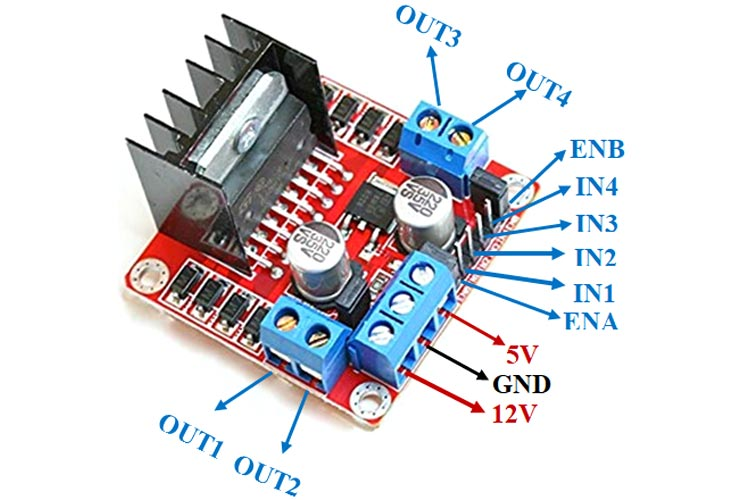
\includegraphics[width=9cm]{./Figures/Motor_driver_L298.jpg}
    \caption{Dual motor driver module (L298N)}
    \label{Motor_driver_L298}
    \end{figure}
    
    \item The two motors are connected at the OUT1/OUT2 and OUT3/OUT4 terminals respectively.
    \item The ENA and ENB pins are for speed control of the two motors. PWM signal generated at the controller end is sent to these pins for motor speed control.
    \item The IN1 and IN2 pins are used for direction control of motor-1, while IN3 and IN4 pins are used for direction control of motor-2.
    \item 12V DC input is routed to the motors using H-bridge inside the L298 IC mounted on the driver module. The motor driver also has a regulator IC which produces 5V output which can be used to drive our micro-controller unit. This eliminate the need for a separate power supply for the micro-controller.
\end{itemize}

A Typical connection between the driver module and the motors is as shown in Figure \ref{Driver_module_connection}. The speed and direction control signals are received from the micro-controller unit.

\begin{figure}[h!]
\centering
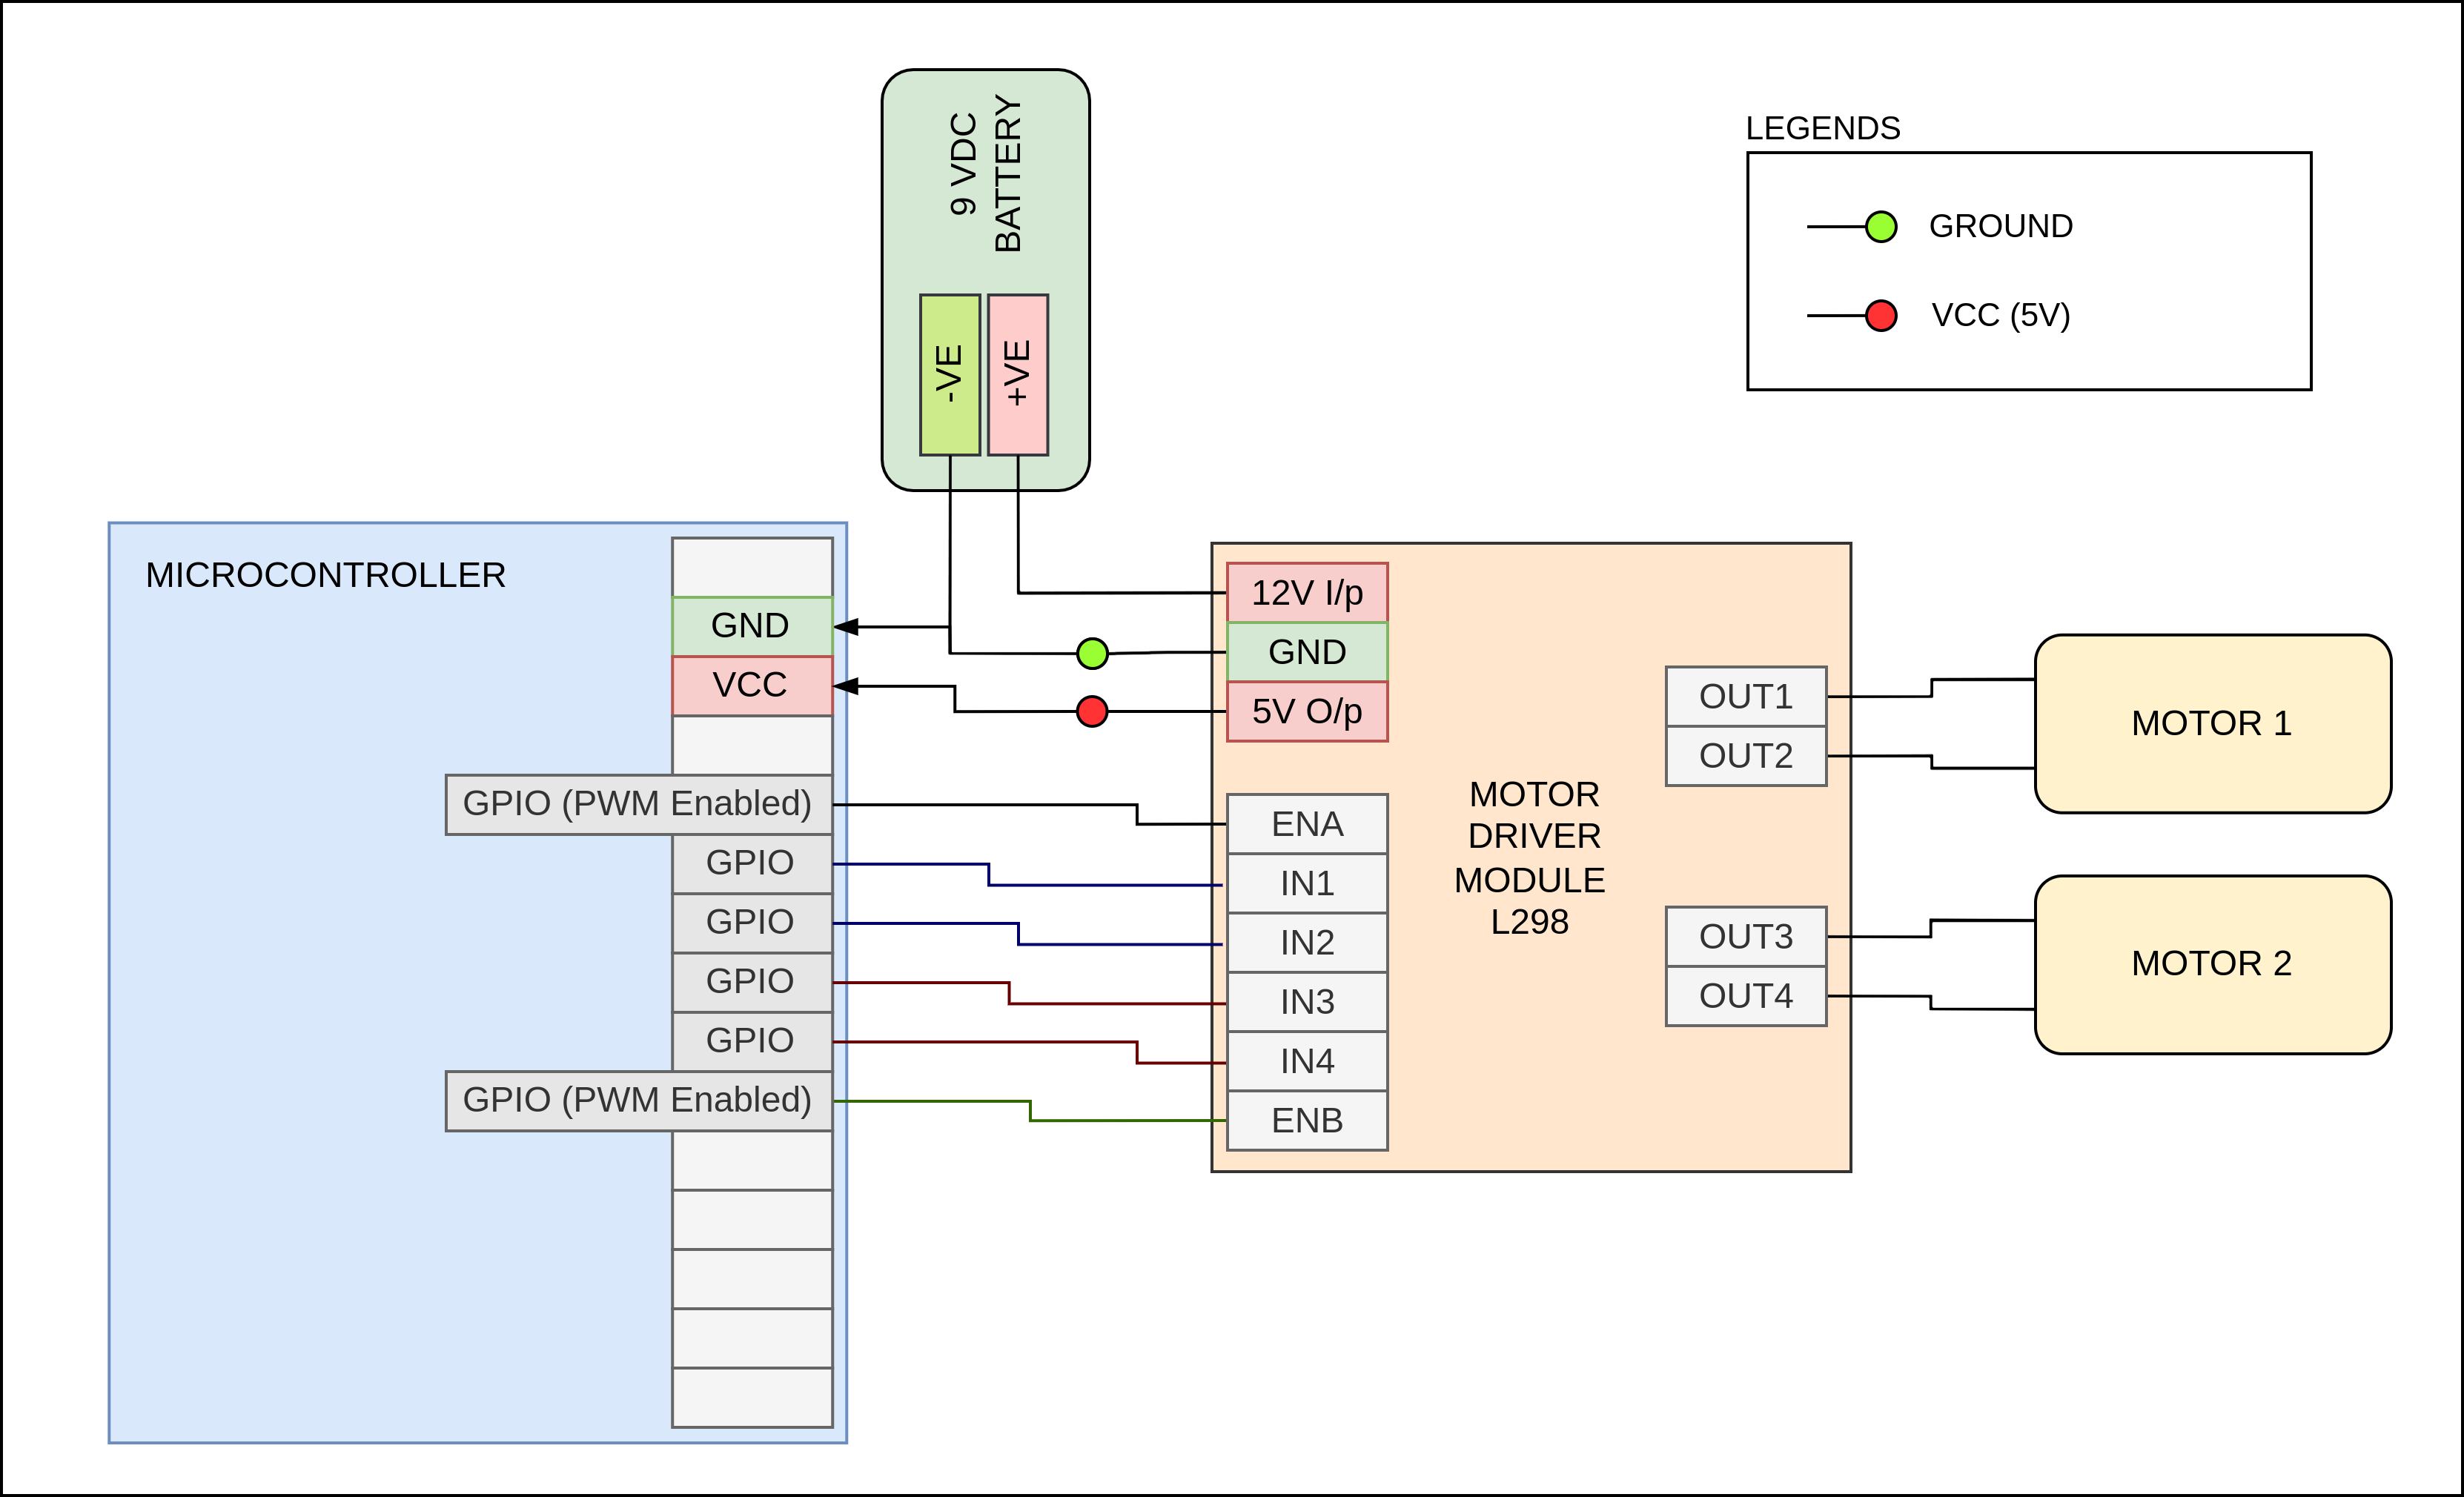
\includegraphics[width=\columnwidth]{./Figures/Driver_module_connection.png}
\caption{Typical connection for motor driver module}
\label{Driver_module_connection}
\end{figure}

\newpage
\section{Brush-less DC motor}
\par BLDC motors primarily consists of two main parts i.e. stator and rotor as shown in Figure xxx. Stator consist of coils made from good conducting materials (copper or aluminium), while rotor is a permanent magnet. When current is passed through coils of stator, a electromagnet is created generating a magnetic field which attracts the permanent magnet (rotor). This is basic principle which gives us rotation of BLDC motors.

\par Generally the opposite coils of stator winded together to provide better torque. BLDC motors comes in various configurations based on number of poles and rotor positioning. Inrunner BLDC motors have rotor part positioned inside stator part, while Outrunner BLDC motors have rotor part positioned outside the stator part as shown in figure \ref{BLDC_runner}.

\begin{figure}[h!]
\centering
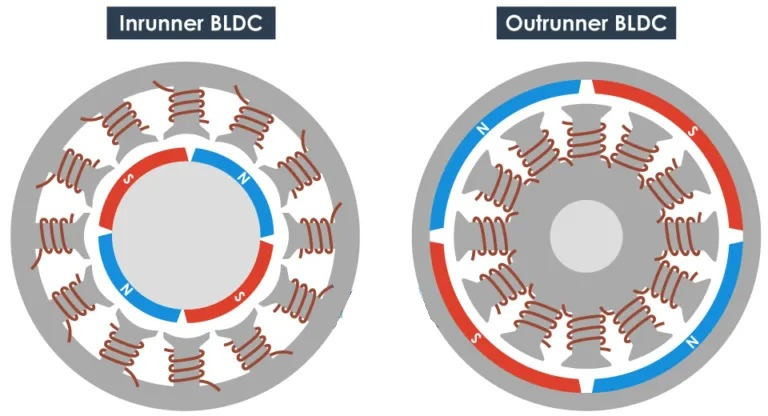
\includegraphics[width=12cm]{./Figures/BLDC_runner.jpg}
\caption{Inrunner BLDC and Outrunner BLDC motors}
\label{BLDC_runner}
\end{figure}

\begin{figure}[h!]
\centering
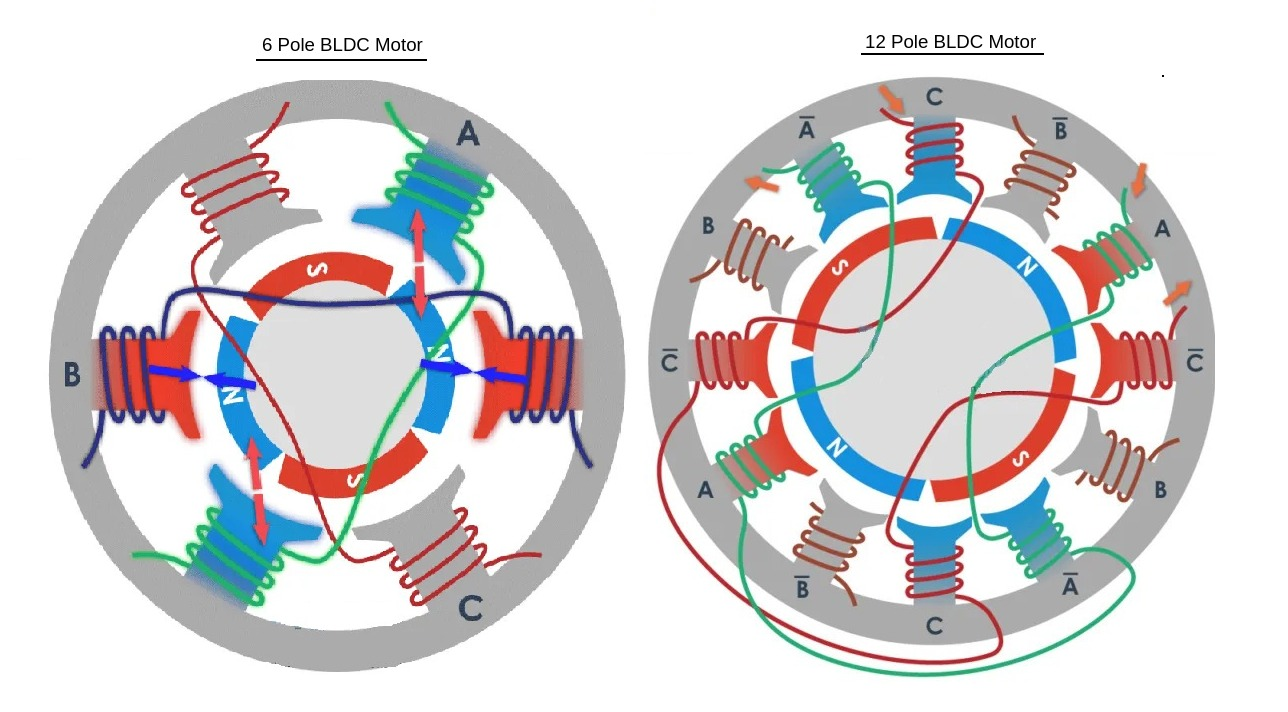
\includegraphics[width=12cm]{./Figures/BLDC_pole.jpg}
\caption{6 Pole and 12 Pole BLDC motors}
\label{BLDC_pole}
\end{figure}

The Electronic speed controller is a device which rotates the BLDC motor by appropriately activating the coils using MOSFET pairs to create rotating magnetic field. Due to MOSFET the switching speed and hence the motor speed can be controlled. The connection between ESC and BLDC motor is as shown in Figure \ref{ESC_BLDC_connection}. Basically, the ESC uses two types of mechanism in order to figure out the position of the stator so that it can decide which coil should be activated for continuous rotation:
\begin{itemize}
    \item Using Hall effect sensor
    \item Back EMF sensing
\end{itemize}

\begin{figure}[h!]
\centering
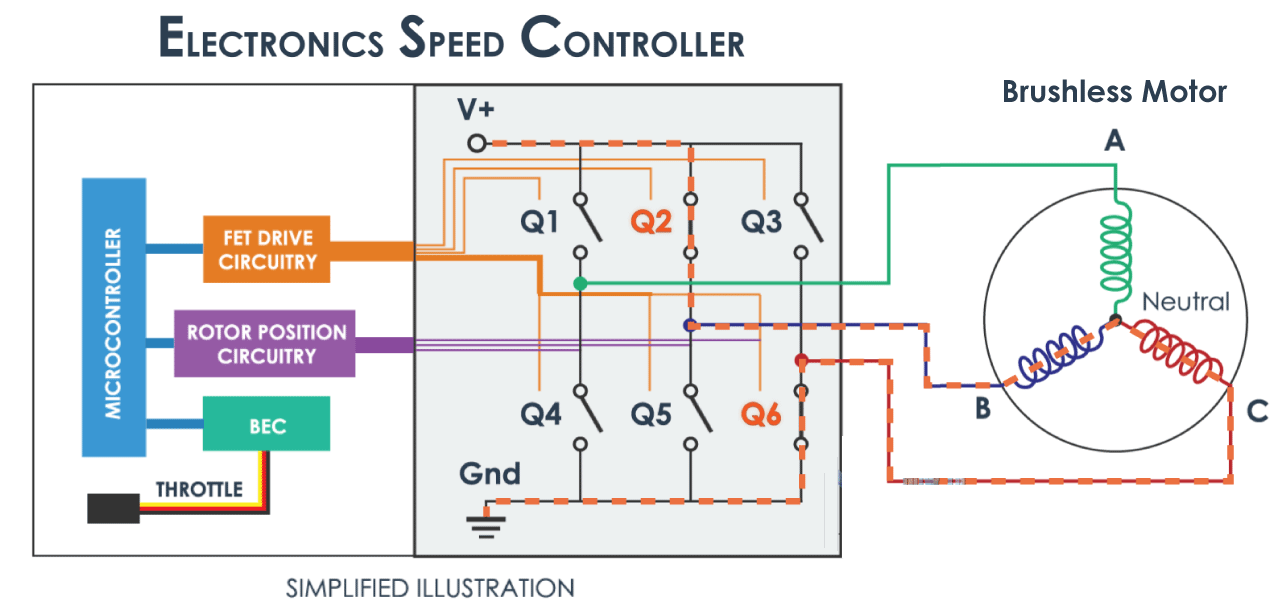
\includegraphics[width=14cm]{./Figures/ESC_BLDC_connection.png}
\caption{Connection between the ESC and BLDC motor}
\label{ESC_BLDC_connection}
\end{figure}

